\section{LSRs and MPLS clusters}\label{cluster}
% %%%%%%%%%%%%%%%%%%%%%%%%%%%%%%%%%%%%%%
This section aims at better
understanding the impact of MPLS deployments over Internet, specifically over
router level topology. To achieve our purpose, we study how LSRs and \dfn{MPLS clusters} 
interacts  with non MPLS routers. Generally speaking, we compare the fingerprints  on $k$-core 
decomposition that MPLS presence causes over the Internet Topology. We propose two main studies: the
first one related to locate the LSRs and MPLS clusters over the entire router topology; and a second
one related to understand the MPLS structure for a given AS.

\subsection{Definitions and Background}\label{cluster.methodo}
% %%%%%%%%%%%%%%%%%%%%%%%%%%%%%%%%%%%%%%
\begin{figure*}[!htb]
  \begin{center}
    \subfigure[Degree Distribution Probability]{\label{fig_degree_distribution}
      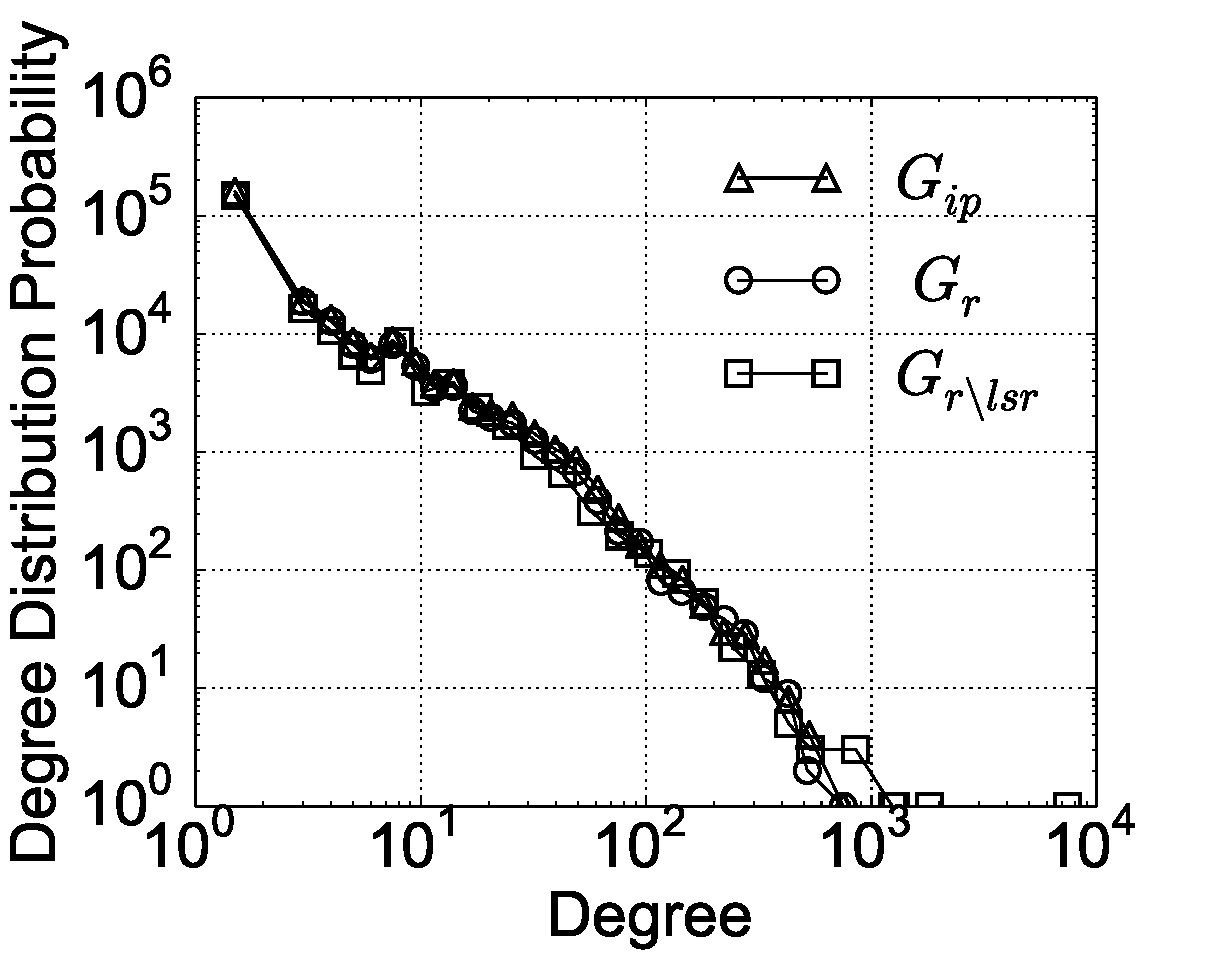
\includegraphics[width=5.5cm]{DegreeDistribution}}\hfil
    \subfigure[Clustering Coefficient]{\label{fig_clustering}
      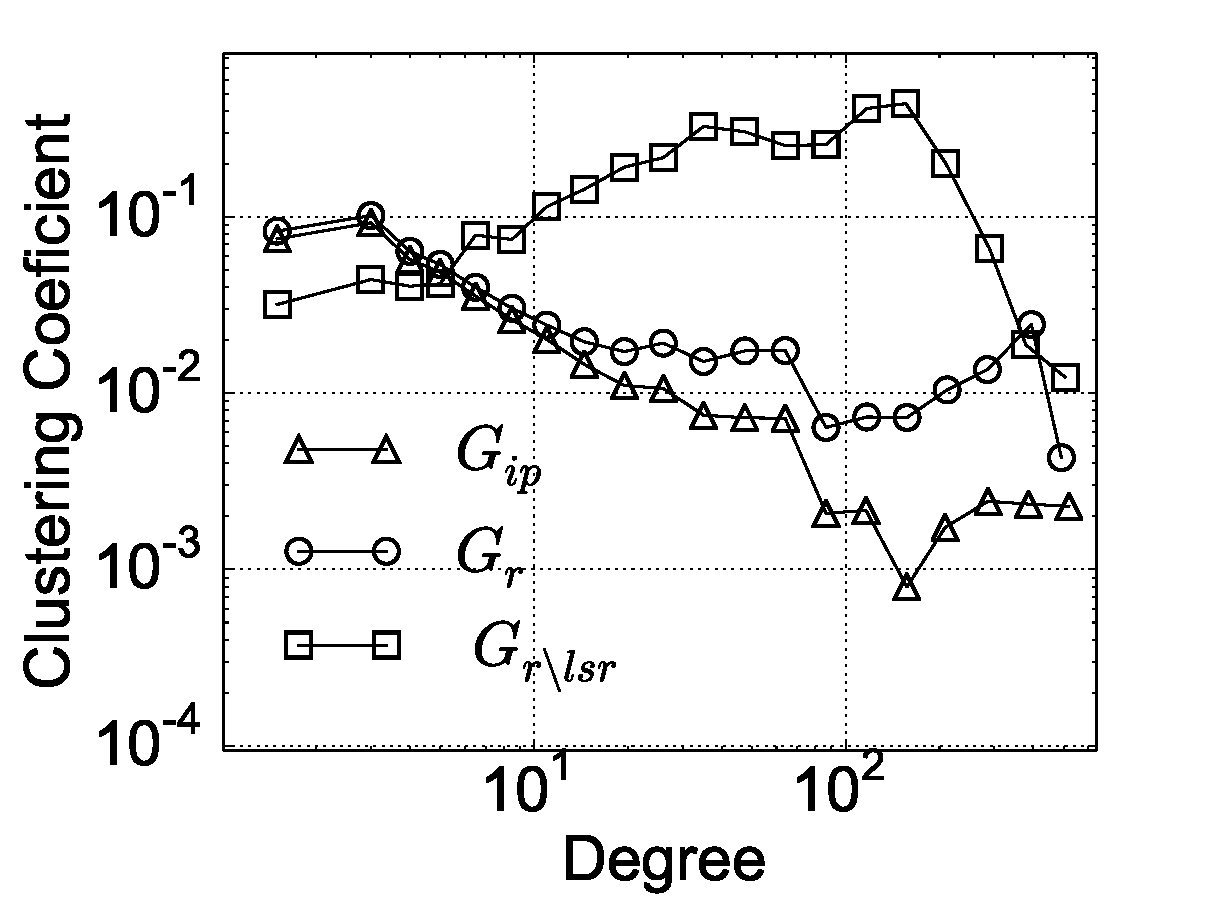
\includegraphics[width=5.5cm]{ClusteringCoeficient}}\hfil
    \subfigure[Neighbor Degree Distribution]{\label{fig_neighbor}
      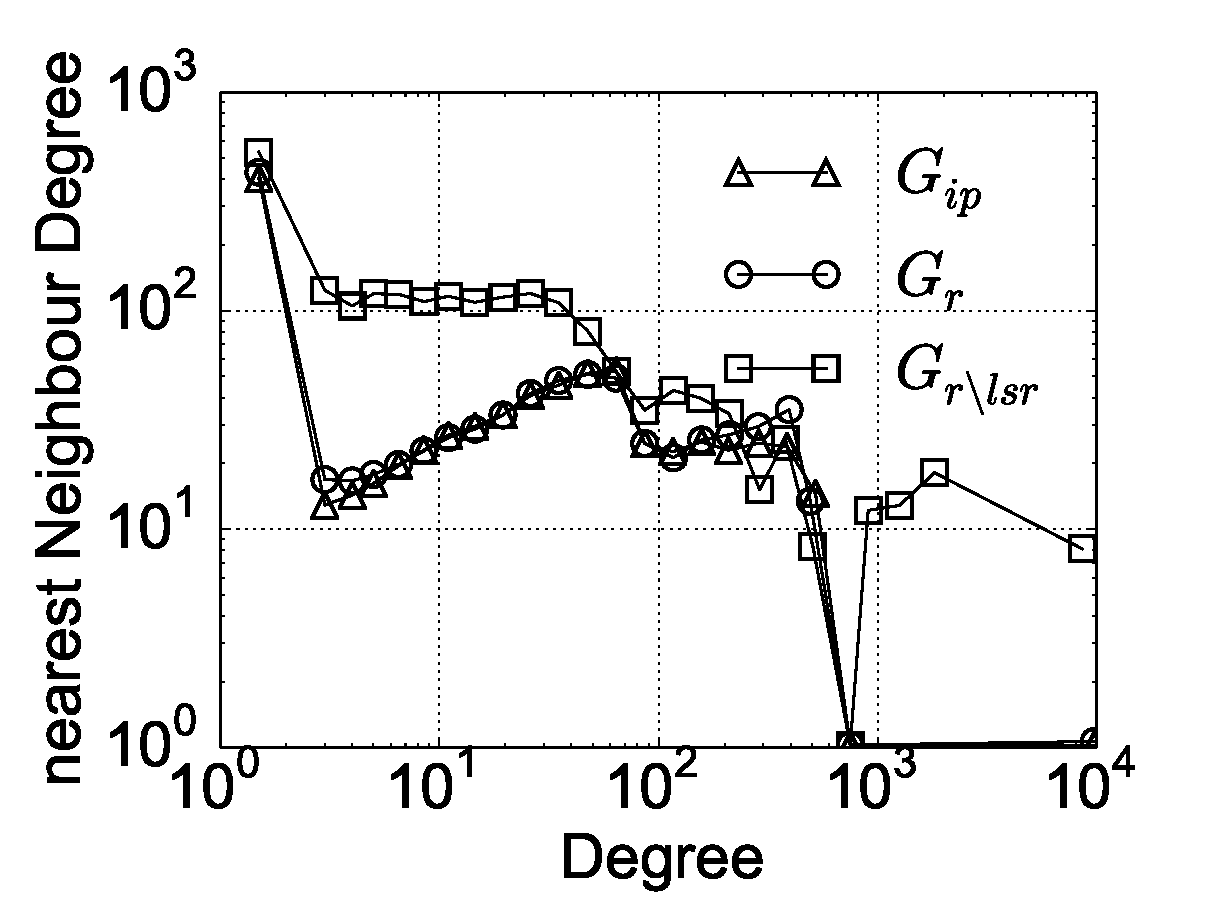
\includegraphics[width=5.5cm]{NearestNeighbor}}
  \end{center}
\caption{Metrics for IP, router and MPLS cluster interconnection
topologies.} 
\label{fig_metrics}
\end{figure*}

\begin{table}[!t]
  \begin{center}
    \begin{tabular}{l|ll}
    \textbf{Graph} & \textbf{Notation} & \textbf{Definition}\\
    \hline
    IP                 & $G_{ip}$ & $(V_{ip}, E_{ip})$\\
    Router             & $G_r$ & $(V_r, E_r)$\\    
    MPLS               & $G_r^{mpls}$ & $(V_r^{mpls}, E_r^{mpls})$\\
    ASes induced graph & $G_r(as)$ & $(V_r(as), E_r(as))$\\    
    %MPLS cluster       & $C_i^{mpls}$ & Connected Component of $G_r^{mpls}(as)$\\
    MPLS cluster interconnection graph & $G_{r \backslash lsr}$ & $(V_{r
    \backslash lsr}, E_{r \backslash lsr}^{mpls})$
    \end{tabular}
  \end{center}
  \caption{Summary of graph notations used in Sec.~\ref{cluster}.}
  \label{cluster.table_notations}
\end{table}

We defined several graphs at different abstraction levels as follows (The main
are summarized in Table~\ref{cluster.table_notations}): First, the \dfn{IP level
graph} $G_{ip}$, built by the IP addresses and links found trough \traceroute.
Second, the \dfn{router level graph} $G_{r}$, getting after solve alias
resolution process through MIDAR~\cite{Keys13}). Third, the \dfn{MPLS router
level graph} $G^{mpls}_{r}$, formed by MPLS links and routers in which at least
one IP interface belongs to an LSP.

The \dfn{ASes induced graph} $G_{r}(as)$ is a subgraph of $G_{r}$ where each
vertex  has an interface belonging to the same Autonomous System, namely $as$.
In particular, the induced graph of $G_r^{mpls}$ is $G^{mpls}_{r}(as)$.
Considering a connected component $C^{mpls}_{i}$ in a $G^{mpls}_{r}(as)$, it is
called  \dfn{MPLS cluster}. Finally, the \dfn{MPLS cluster interconnection
graph} is an hybrid router level graph,  $G_{r\backslash lsr}$, where all the
MPLS clusters $C^{mpls}_{i}$ are gathered together in a single node, while
non-MPLS capable routers remain unchanged. Broadly speaking, an MPLS cluster
interconnection graph refers to a router level graph where all MPLS clusters are
treated as a single node. Additionally, we call $G_{r\backslash lsr}(as)$ to the
induced subgraphs of $G_{r\backslash lsr}$ by routers having at least one
interface in the Autonomous System $as$.

This work,  principally focused on MPLS clusters interconnection graph
$G_{r\backslash lsr}$ and their respective ASes induced graphs $G_{r\backslash
lsr}(as)$. In this way, we study how MPLS clusters are connected to non-MPLS
capable routers. Particularly, as MPLS clusters interconnection graph analysis
is mainly based on $k$-core decomposition, we  present the following
definitions:
\begin{itemize}
  \item\dfn{\textit{k}-core:} Given a graph $G=(V,E)$, then the
  subgraph $H=(C,E|C)$ induced by the set $ C\subseteq V$ is a \textit{k}-core
  of order $k$ $iff$ $\forall v \in C: degree_{H}(v)\geq k$ and $H$ is the
  maximum subgraph with this property.
      
  \item\dfn{Shell index}. A vertex $i$ has a shell index $c$ if it
  belongs to the $c$-core but not to $(c+1)$-core. We denote by $C_i$ the shell
  index of vertex $i$. A shell $C_c$ consists of all the vertices whose shell
  index is $c$. The maximum value $c$ such that $C_c$ is not empty is denoted by
  $C_{\max}$.  Therefore, the $k$-core is thus the union of all shells $C_c$ with
  $c \geq k$.
\end{itemize}

To retrieve the $k$-core decomposition of a graph $G$, we use
\lanet\cite{Alvarez06k}. This tool returns a two dimensional plot, where the
position of each vertex is arranged into a circle depending on its shell index
and its neighbors' index. A color code allows for the identification of shell
indices, and diameter of the spheres represent vertex's degree in a logarithmic
scale. The $k$-core decomposition can break the original network into various
connected components which are displayed as independent circles.

\subsection{MPLS on Internet Topology}\label{cluster.topo}
% %%%%%%%%%%%%%%%%%%%%%%%%%%%%%%%%%%%%%%
\begin{figure}[!t]
  \begin{center}
    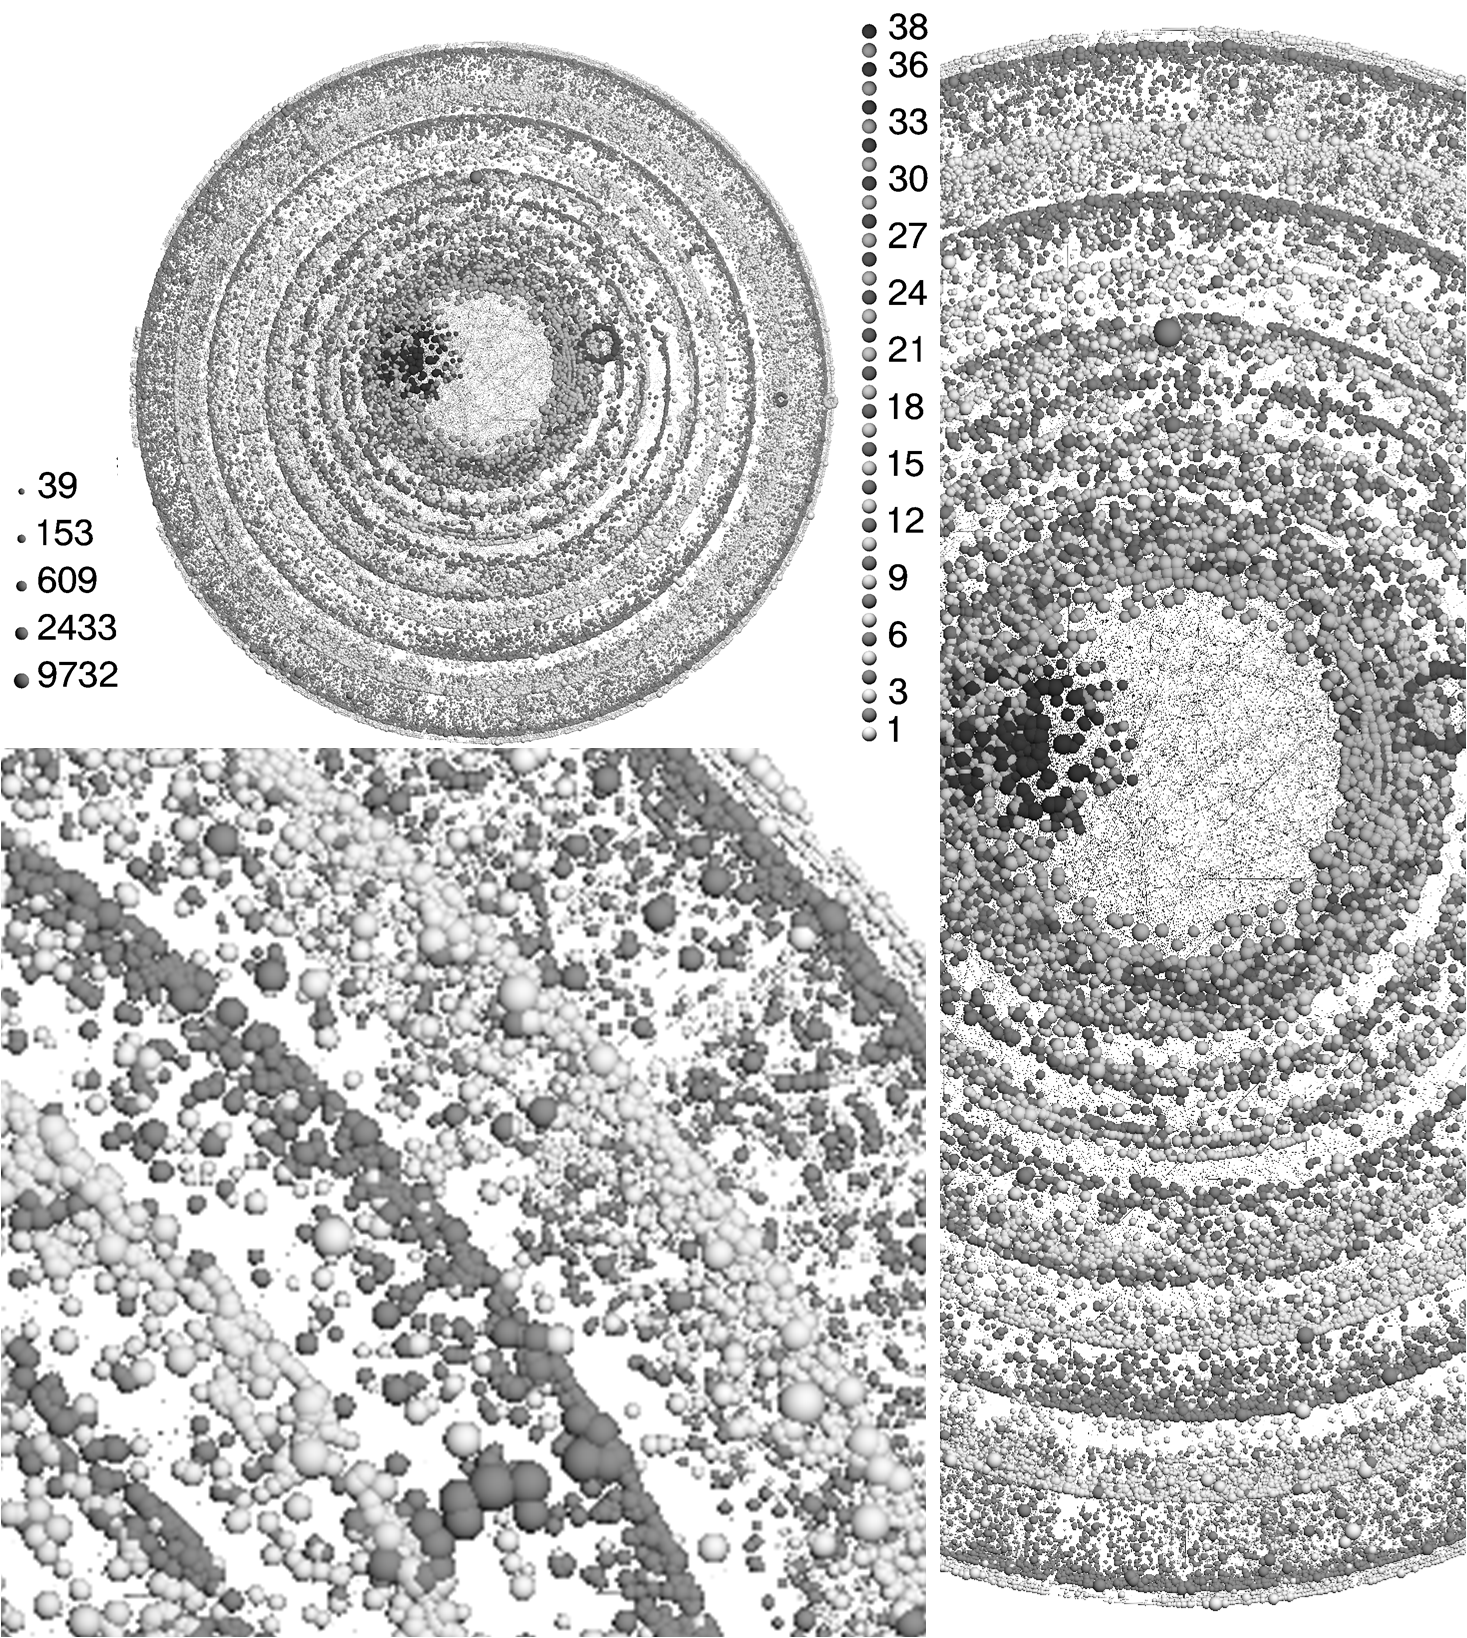
\includegraphics[width=3in]{Routers}
  \end{center}
  \caption{$k$-core visualization of router level topology $G_{r}$.}
  \label{fig_k_core_routers}
\end{figure}

In this section we study the LSRs and MPLS cluster structure over the Internet
Topology.  First, we selected the router level topology for our analysis because
it is closer to a realistic Internet one and because  we did not notice any
strong difference between IP and router level topology as Fig.~\ref{fig_metrics}
suggests. Indeed, we just noticed that router level topology has slightly
stronger clustering coefficient (see Fig.~\ref{fig_clustering}), due to alias
resolution process. In this way, Fig.~\ref{fig_k_core_routers} shows the
$k$-core visualization of $G_{r}$.  The figure is divided in three parts, the
main part being in the upper left while the two others are a zoom on the main
part.  The main part is composed of two scales, the one on the left is the node
degree scale representing the degree in a logarithmic scale, while the one on
the right is a gray scale with each shell index $c_i$. Between the two scales,
we see the shell index with $C_{\max}$ in the center, the other shells being
located concentrically around it. Note that $C_{\max}$-core is made of several components with one
having the most significant part, and it is shown at the left of the center
(black nodes).  We also see that all the shells index are highly populated and
that the node degree is not related with the shell index, i.e., there are many
routers with high degree in the outer (lower) shells.  Another typical feature
of router level topology is that the links between routers mainly occurs between
routers belonging to neighbors shells, e.g., the routers on the outer shells are
not usually connected to the routers located on the  $C_{\max}$-core, as it is
in the Autonomous Systems maps~\cite{Alvarez06k}.

\begin{figure*}[!t]
  \begin{center}
    \subfigure[The $k$-core visualization of router level topology $G_{r}$.]{\label{fig_k_core_LSR}
      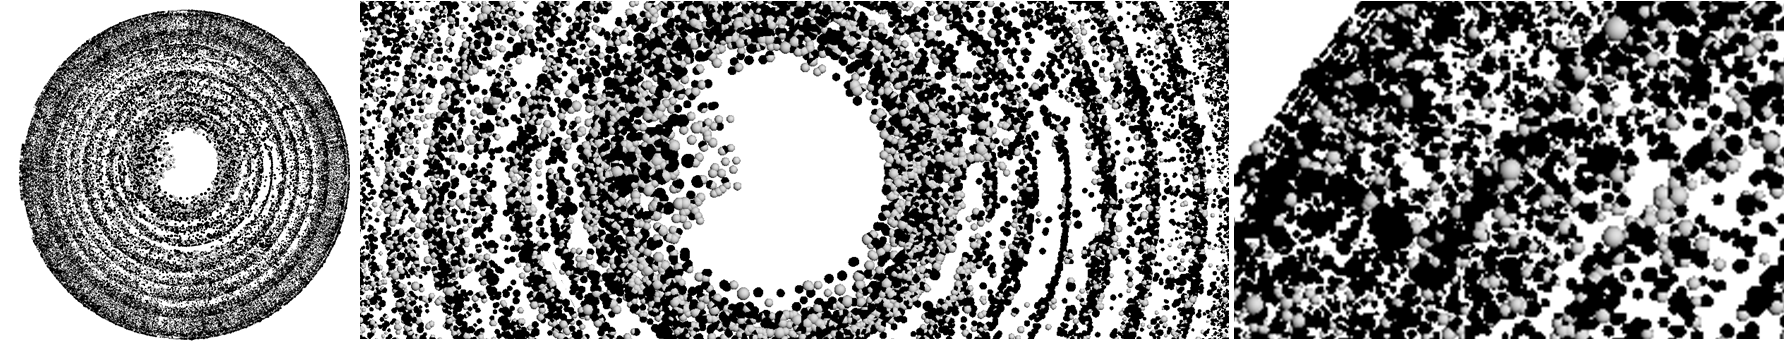
\includegraphics[width=18cm]{LSR}}
\hfil
    \subfigure[The $k$-core visualization of MPLS cluster level topology  $G_{r\backslash lsr}$.]{\label{fig_k_core_MPLS}
      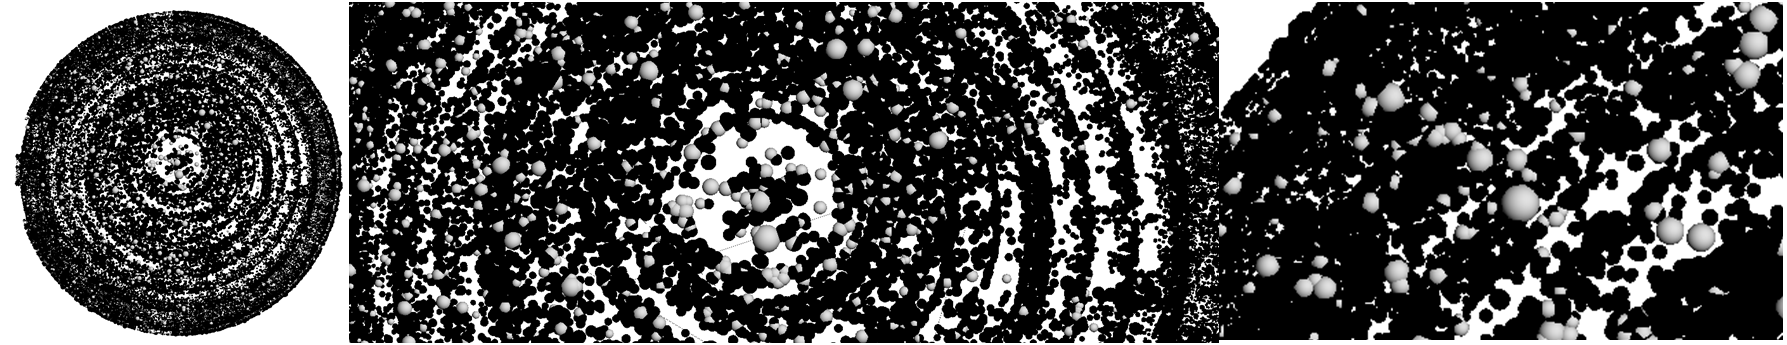
\includegraphics[width=18cm]{MPLS}}
  \end{center}
  \caption{$k$-core visualization of $G_r$ and $G_{r \backslash lsr}$.  On
  Fig.~\ref{fig_k_core_LSR}, black nodes refer to non MPLS capable routers and
  gray nodes refer to LSRs.  On Fig.~\ref{fig_k_core_MPLS}, black nodes refer to
  non MPLS capable routers and gray nodes refer to MPLS clusters.} 
  \label{fig_kcore_overview}
\end{figure*}

In order to locate LSRs-routers with MPLS capabilities into the shells index
over $k$-core decomposition, we paint in black the non-MPLS routers and in gray
the LSRs. The results are showed in Fig.~\ref{fig_k_core_LSR}.  For the sake of
the visualization, we do not include neither the shell index, degree scale, nor
edges between shells. We notice that the LSRs are commonly distributed around
the different shells of Internet, with slightly low density in the lower shells.
Additionally, we apply the same methodology for the MPLS interconnection cluster
level graph $G_{r\backslash lsr}$ (Fig.~\ref{fig_k_core_MPLS}): MPLS clusters
(gray nodes) are distinguished from the non-MPLS capable routers (black nodes).
In this case,  MPLS clusters  degree is correlated with shell index: as higher
is shell cluster then higher is its degree. This behavior is observed in
hierarchical networks, e.g., the Autonomous System network.


Finally, we evaluate $G_{r \backslash lsr }$ using metrics such as degree
distribution, clustering coefficient, and nearest neighbor degree, as is shown
on Fig.~\ref{fig_metrics}. We notice that MPLS clusters highly impact over the
router level topology. On one hand, the nearest neighbor degree highly
increments for low degrees nodes on $G_{r \backslash lsr}$, suggesting that
routers with low degree are highly connected to MPLS clusters and thereby to
LSRs. Notice that vertices with high degree are principally the MPLS clusters,
as Fig.~\ref{fig_k_core_MPLS} shows. On the other hand, the clustering
coefficient of $G_{r \backslash lsr }$ is highly increased for vertices having
degree $50$ to $200$. This suggests that MPLS deployments plays an important
role on Internet robustness, i.e., local robustness of the network increase
because there exists different paths joining every pair of close vertices
(higher clustering means more triangles in the network).

\subsection{MPLS clusters on Autonomous Systems}\label{cluster.as}
% %%%%%%%%%%%%%%%%%%%%%%%%%%%%%%%%%%%%%%%%%%%%%%%%%%%%%%%%%
Although, the previous results give us a general overview about MPLS deployment,
we believe that the study of MPLS structure requires to go deeper into the
individual AS topology. Indeed, we found that around $89.9\%$ of MPLS links are
intra-domain. Thereby, we focus on the top ASes in terms of total number of
discovered links.  On this set of ASes, we discard those having less than 500
MPLS links. Additionally, we identify the amount of discovered MPLS links by AS,
distinguishing the type of MPLS tunnel to their belong, i.e., given a link
between two MPLS interfaces $i_{n-1}$  and $i_{n}$ discovered by traceroute at
$n-1$ and $n$ position, we called:

\begin{itemize}
  \item[i] \dfn{explicit MPLS link:} links 
  where $i_{n}$ belongs  to an explicit MPLS tunnel.
  \item[ii] \dfn{qTTL MPLS link:} links 
  where $i_{n}$ belongs  to an implicit MPLS tunnel qTTL based.
  \item[iii] \dfn{u-turn MPLS link:} links 
  where $i_{n}$ belongs  to an implicit MPLS tunnel u-turn based.
\end{itemize}

The summary of the top ASes is showed in the Fig.~\ref{top_as}.
We noticed that the ratio $r_{mpls}= \vert E^{mpls}_{r} (as) \vert /\vert E_{r}
(as) \vert $  is greater when more explicit MPLS links have been discovered.
Interestingly, we also see that the ASes with more IP links discovered have the
lowest ratio $r_{mpls}$. For our purposes, we select the most representatives
ASes from those in Fig.~\ref{top_as}. In this way, we analyzed the graphs
$G_{r}(as)$ and $G_{r\backslash lsr}(as)$ for AS1299, AS174, AS6762, AS2914,
AS7018 and AS1273 using  $k$-core decomposition (see Fig.~\ref{fig_cluster_mpls}).
We observed that  $k$-core decomposition structure varies according
the type of MPLS tunnels that prevails in the AS. Particularly, for  AS1299 (Teliasonera AB), AS174 (Cogent Communication) and AS6762 (Telecom Italia) where prevails u-turn MPLS links,
we show that MPLS clusters (represented as gray nodes)  are spread out over different shells. These $k$-core structures are similar in our top five of ASes where u-turn signature was majority
discovered, i.e., between $30\%$ and  $80\%$ over  the total amount of MPLS
links. 

However, for  AS2914 (NTT America Inc.), AS7018 (AT\&T) and AS1273 (Cable and
Wireless Worldwide plc) where prevail explicit MPLS links, we found a $k$-core
structure highly different, i.e., Most of vertices are directly connect to a
predominant MPLS cluster located at $C_{\max}$-core. The remain of  ASes in
Fig.~\ref{top_as} with high percentage of explicit tunnels have the same
structure.

Summarizing, we notice that ASes where prevails explicit MPLS links has a 
predominant MPLS cluster while ASes where prevails u-turn MPLS links have several MPLS cluster spread out over the shells. 
Additionally, We believe that $k$-core decomposition  on the top five ASes could have different structure due to either  the u-turn signature inaccuracy or due to some particular MPLS
deployment. Indeed, we noticed only on these ASes a low ratio $r_{mpls}$ and an
unusual  high presence of  u-turn links.

Another remarkable observation  relays on the fact that the maximum degree
reached by MPLS clusters is considerably high in regard to the network
size. Indeed, with exception of AS174, the rest of ASes suggest that more than
$50\%$ of non-MPLS routers are connected  to at least one LSR. Actually, even
the outer shells of the $k$-core decomposition are linked directly with the
MPLS clusters located in the $C_{\max}$-core. This behavior match with
our observation of nearest neighbor degree and clustering coefficient noticed on
Sec.~\ref{cluster.topo}. Additionally, because MPLS clusters are
mainly located on $C_{\max}$-core (even on the ASes with high percentage of
u-turn MPLS links), we believe that MPLS plays an important role in the
backbone of the ISPs.

\begin{figure}[!htb]
  \begin{center}
    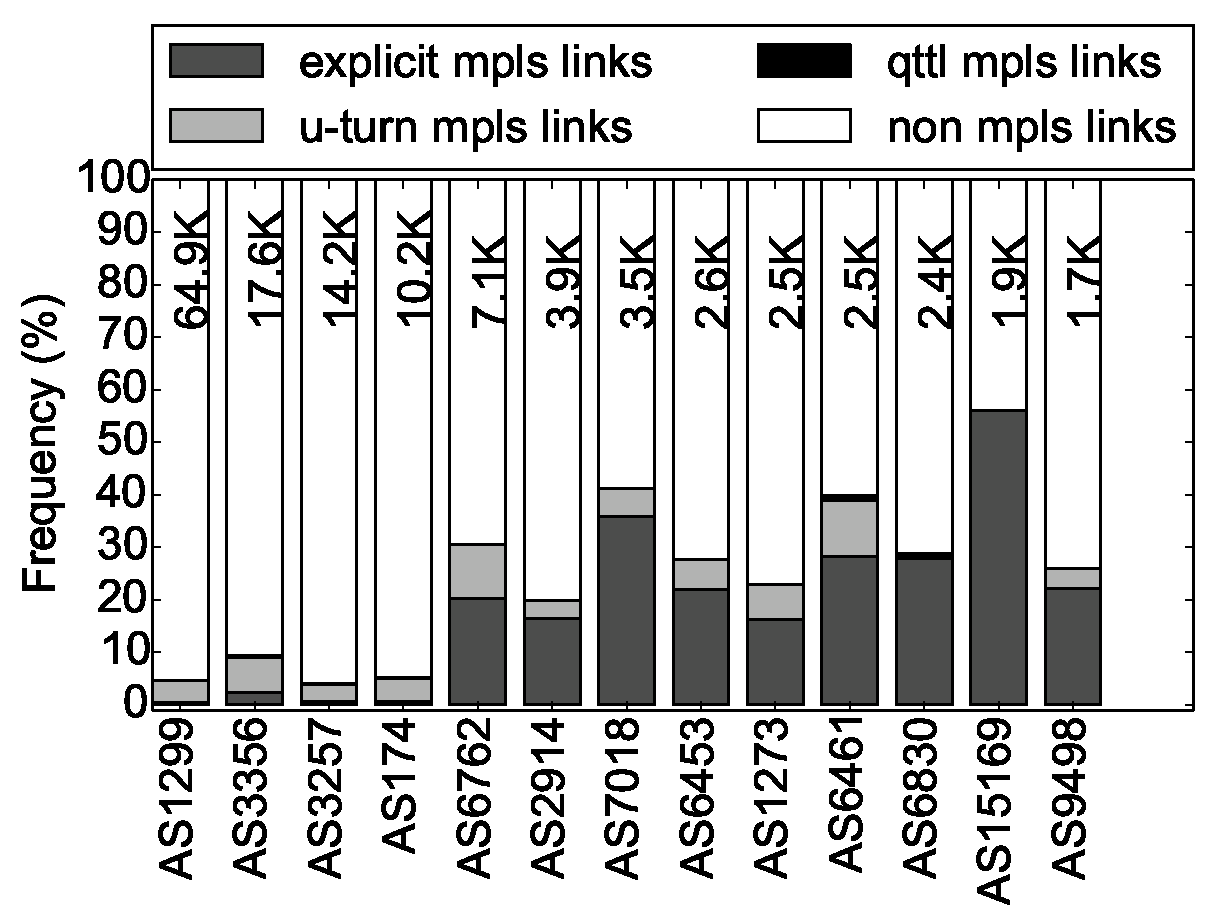
\includegraphics[width=6cm]{TOP_AS}
  \end{center}
  \caption{Top of ASes with most links discovered}
  \label{top_as}
\end{figure}

%Figura u-turn
\begin{figure*}[!htb]
  \begin{center}
    \subfigure[AS1299  Teliasonera AB , $C_{\max}=21$, $\text{Degree}_{\max}=2781$, $|V_{r
    \backslash lsr}|=4128$, $|E_{r \backslash lsr}|=24865$ ]{\label{fig_cluster_mpls_1299}
      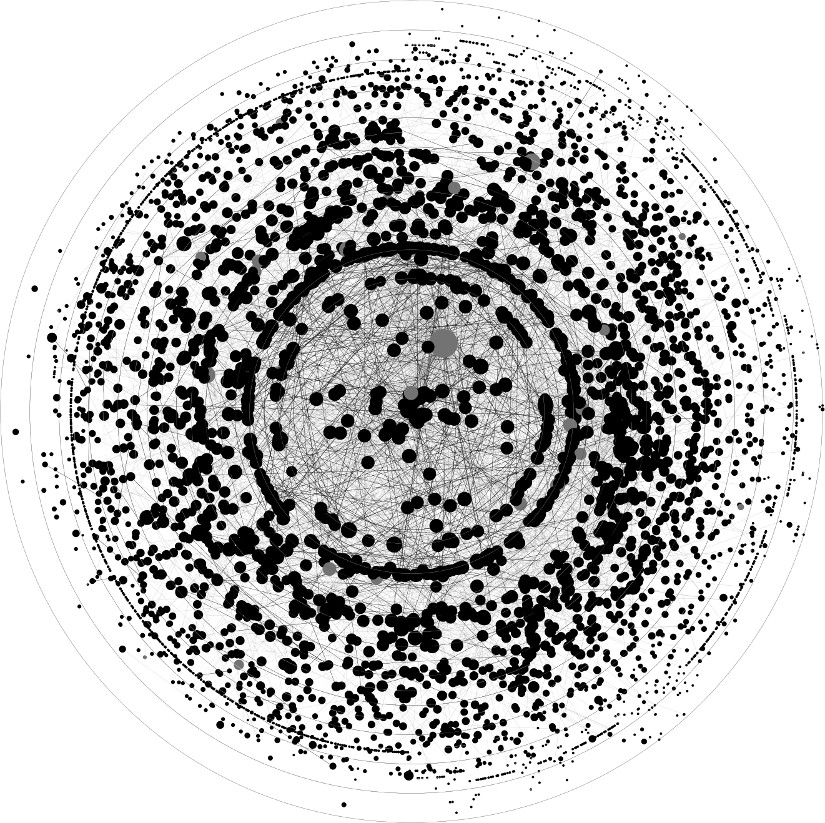
\includegraphics[width=2in]{1299}}
\hfill
    \subfigure[AS174 Cogent Communication, $C_{\max}=8$, $\text{Degree}_{\max}=751$, $|V_{r
    \backslash lsr}|=4421$, $|E_{r \backslash lsr}|=8611$]{\label{fig_cluster_mpls_174}
      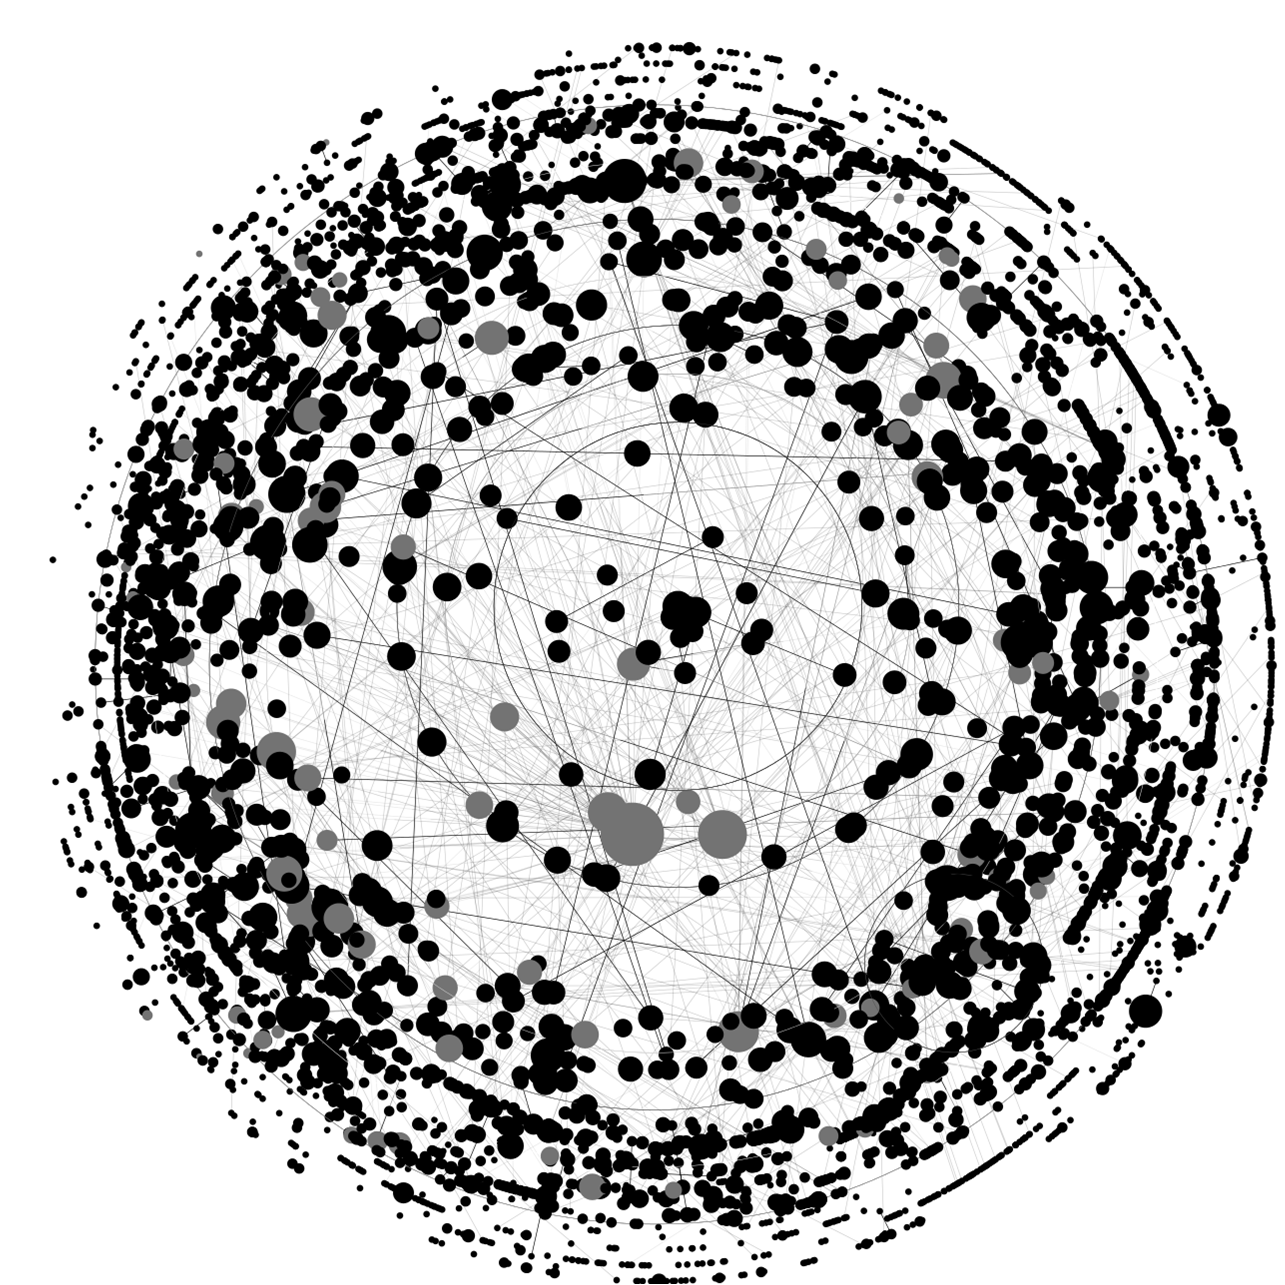
\includegraphics[width=2in]{174}}
\hfill
    \subfigure[AS6762 Telecom Italia, $C_{\max}=10$, $\text{Degree}_{\max}=564$, $|V_{r
    \backslash lsr}|=750$, $|E_{r \backslash lsr}|=1504$]{\label{fig_cluster_mpls_6762}
      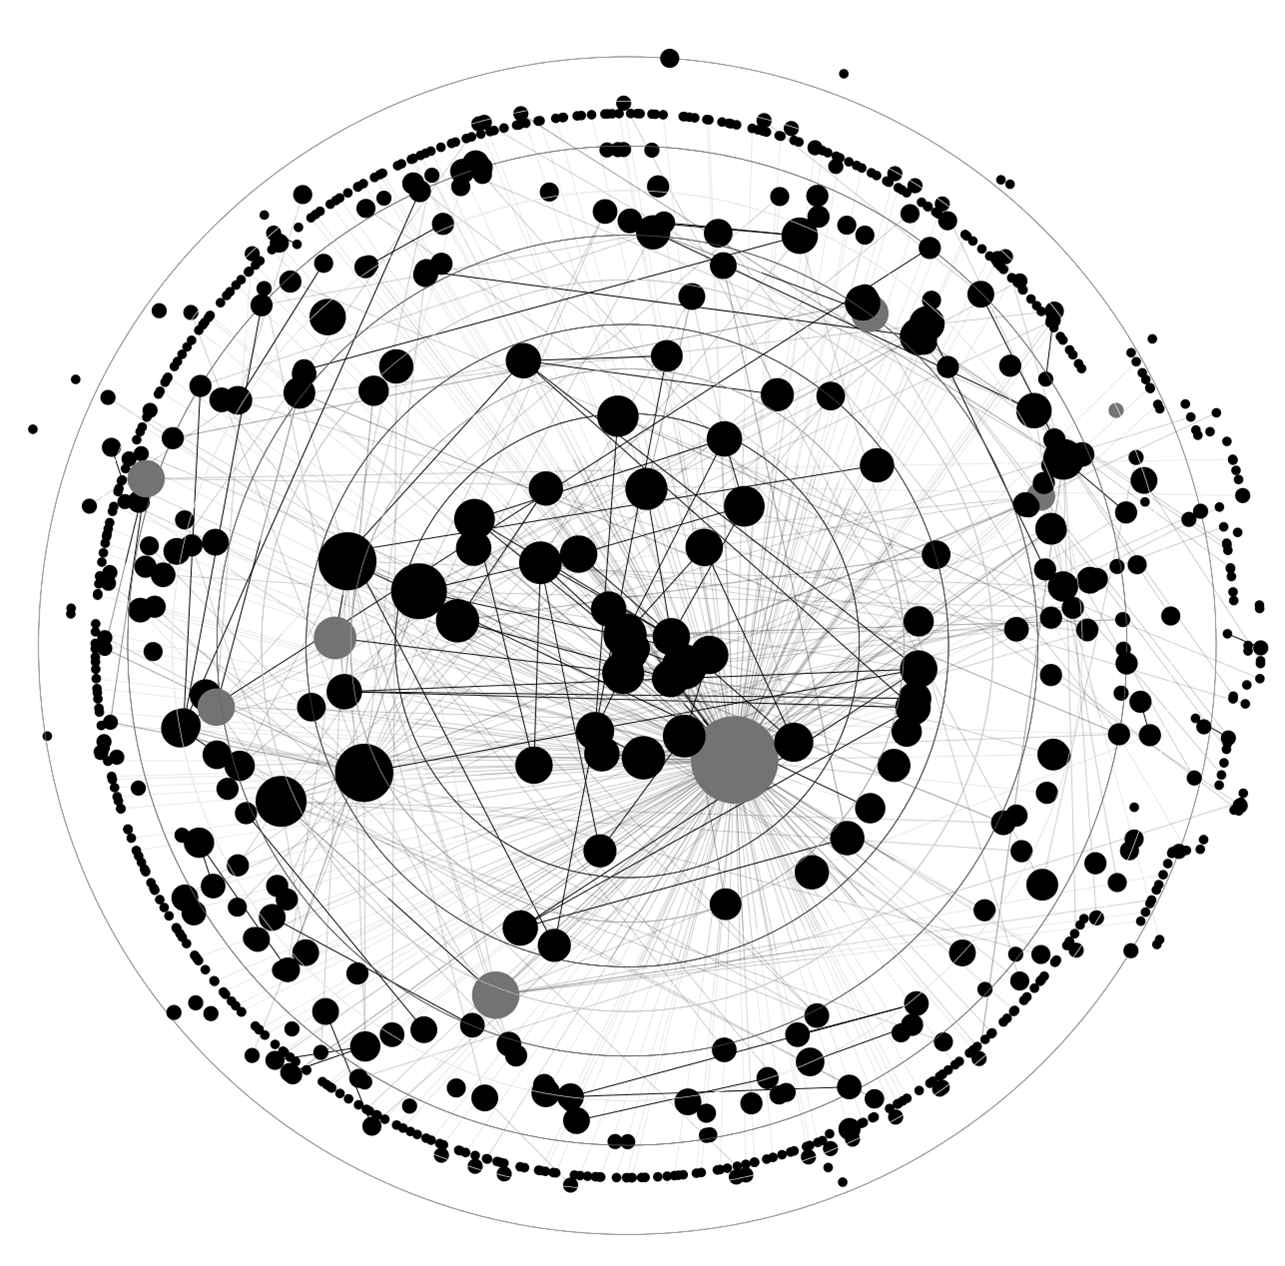
\includegraphics[width=2in]{6762}}
\hfill
    \subfigure[AS2914 NTT America Inc., $C_{\max}=4$, $\text{Degree}_{\max}=1019$, $|V_{r
    \backslash lsr}|=1807$, $|E_{r \backslash lsr}|=2360$]{\label{fig_cluster_mpls_2914}
      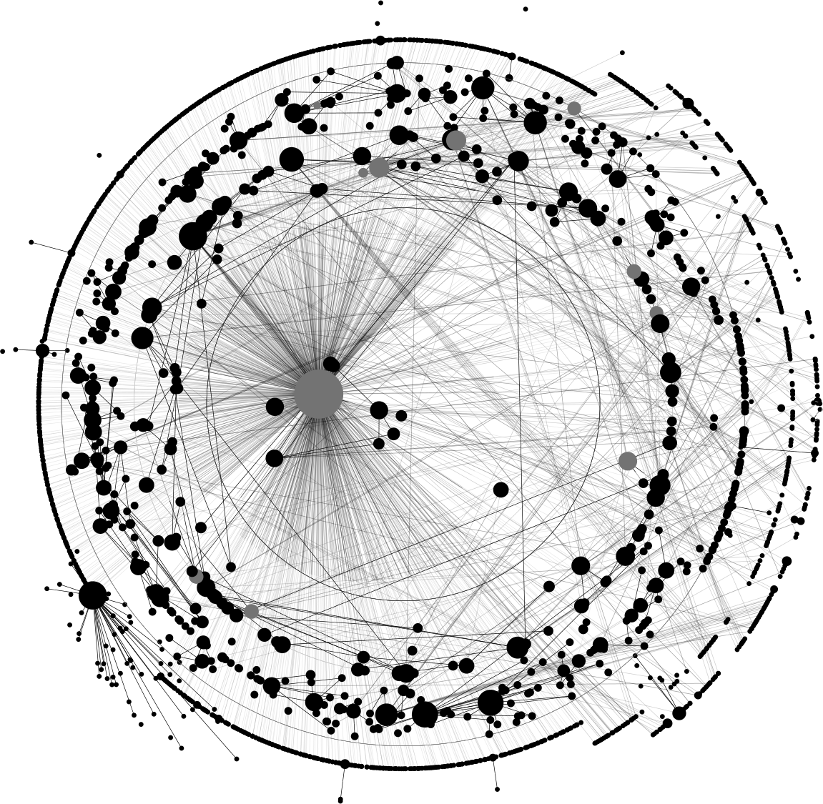
\includegraphics[width=2in]{2914}}
\hfil
    \subfigure[ AS7018 AT\&T, $C_{\max}=3$, $\text{Degree}_{\max}=745$, $|V_{r
    \backslash lsr}|=1306$, $|E_{r \backslash lsr}|=1441$]{\label{fig_cluster_mpls_7018}
      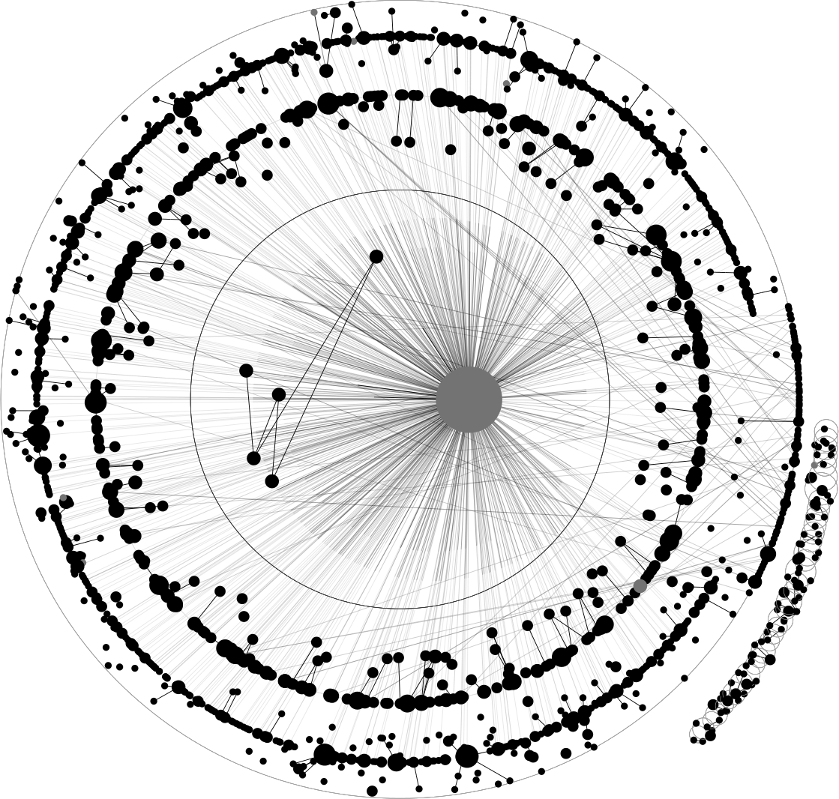
\includegraphics[width=2in]{7018}}
\hfil
    \subfigure[ AS1273 Cable and Wireless Worldwide plc, $C_{\max}=3$, $\text{Degree}_{\max}=806$, $| V_{r \backslash lsr}|=1127$, $|E_{r \backslash lsr}=1215$]{\label{fig_cluster_mpls_1273}
      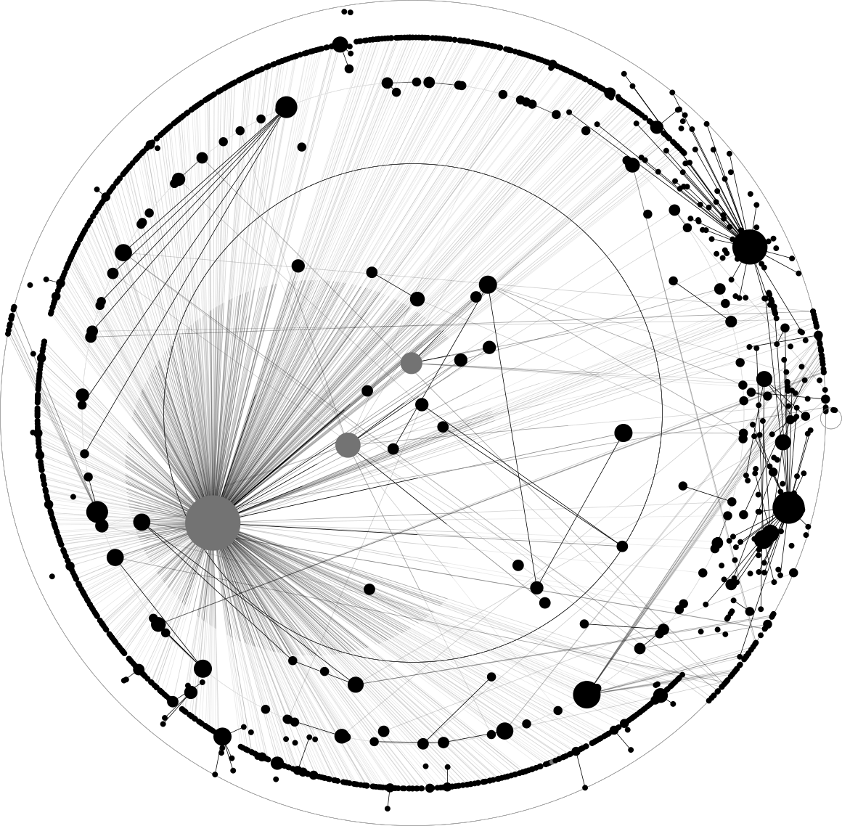
\includegraphics[width=2in]{1273}}
  \end{center}
  \caption{$k$-core visualization of MPLS cluster interconnection Graph
  $G_{r\backslash lsr}(as)$. On the top, the ASes show several MPLS clusters
  spread out around the shells. On the bottom, the ASes
  show a predominant MPLS cluster located on
  $C_{\max}$.}
  \label{fig_cluster_mpls}
\end{figure*}